\documentclass{szzclass}

\usepackage{amsmath}
\usepackage{graphics}
\usepackage[export]{adjustbox}[2011/08/13]
% \usepackage[czech]{babel}
% \usepackage[margin=3cm]{geometry}
% \usepackage{wrapfig}

% spacing
\usepackage{titlesec}
% \titlespacing*{\section}{0pt}{1ex}{0.5ex}
\titlespacing*{\subsection}{0pt}{1ex}{0ex}

% \topic{Modulární aritmetika, základy teorie čísel, Malá   Fermatova věta, diofantické rovnice, lineární kongruence, Čínská věta o   zbytcích.}
\title{Modulární aritmetika, základy teorie čísel, Malá   Fermatova věta, diofantické rovnice, lineární kongruence, Čínská věta o   zbytcích.}
\renewcommand*\contentsname{Obsah}
\author{Daniel Hampl}
% \code{BI-SPOL-33}
% \subject{ZDM}

\begin{document}
\maketitle

\tableofcontents
\newpage

\section{Modulární aritmetika}
$Z_m$ (nebo též $Z mod m$) je množina celých čísel modulo nějaké dané přirozené číslo $m$. Nejčastěji se
setkáme se zápisem $Zm = \{0, 1, 2 . . . , m - 1\}$.

Nechť $a, b, c, d, m \in Z$, $m \geq 2$. Pak pokud platí současně $a \equiv b \text{ mod } m$ a $c \equiv d \text{ mod } m$, potom platí:

\begin{center}
$a + c \equiv b + d \text{ mod } m$

$a - c \equiv b - d \text{ mod } m$

$a \cdot c \equiv b \cdot d \text{ mod } m$
\end{center}

Nechť $a, b \in Z$. Řekneme, že $a$ dělí $b$, značíme $a|b$, jestliže
existuje $k \in Z$ takové, že $b = k \cdot a$.

Vlastnosti
\begin{itemize}
    \item uzavřenost $a$ \textcircled{$+$} $b \in Z_m$, $a$ \textcircled{$\cdot$} $b \in Z_m$
    \item komutativita $a$ \textcircled{$+$} $b = b$ \textcircled{$+$} $a$, $a$ \textcircled{$\cdot$} $b = b$ \textcircled{$\cdot$} $a$
    \item asociativita $a$ \textcircled{$+$} $(b$ \textcircled{$+$} $c) = (a$ \textcircled{$+$} $b)$ \textcircled{$+$} $c$,
    $a$ \textcircled{$\cdot$} $(b$ \textcircled{$\cdot$} $c) = (a$ \textcircled{$\cdot$} $b)$ \textcircled{$\cdot$} $c$
    \item neutrální prvek $a$ \textcircled{$+$} $0 = |a|_m$, $a \cdot 1 = |a|_m$
    \item inv. prvek $a$ \textcircled{$+$} $\bar{a} = 0$
    \item distributivita $a$ \textcircled{$\cdot$} $(b$ \textcircled{$+$} $c) = a$ \textcircled{$\cdot$} $b$ \textcircled{$+$} $a$ \textcircled{$\cdot$} $c$
\end{itemize}

\newpage

\section{GCD \& LCM}
Číslo $d \in N^+$ je společný dělitel čísel $a$, $b$, jestliže $d|a$ a $d|b$. Největší z nich je poté gcd$(a,b)$.

Číslo $n \in N^+$ je společný násobek čísel $a$, $b$, jestliže $a|n$ a $b|n$. Nejmenší z nich je poté lcm$(a,b)$.

(Vlastnosti gcd a lcm). Nechť $a$, $b$ $\in Z$. Potom platí:
\begin{itemize}
    \item Jestliže je n společný násobek $a$, $b$, pak $\text{lcm}(a, b)$ dělí $n$.
    \item Jestliže $a|n$ a $b|n$, pak $\text{lcm}(a, b)|n$.
    \item $\text{gcd}(a, b) = \text{gcd}(|a|, |b|)$ a $\text{lcm}(a, b) = \text{lcm}(|a|, |b|)$.
    \item Označme $d = \text{gcd}(a, b)$. Potom $\text{gcd}( a d,bd) = 1$.
    \item $\text{gcd}(a + cb, b) = \text{gcd}(a, b)$ pro libovolné $c \in Z$.
    \item Jestliže $a|bc$, pro nějaké $c \in Z$ a čísla $a$, $b$ jsou nesoudělná (tj. $\text{gcd}(a, b) = 1$), potom $a|c$.
    \item $|a|\cdot|b| = \text{gcd}(a,b) \cdot \text{lcm}(a,b)$
\begin{center}
$\text{gcd}(a, b) = d = \alpha \cdot a + \beta \cdot b$,
\end{center}
kde $\alpha$, $\beta$ jsou celočíselné koeficienty této lineární kombinace.
\end{itemize}

\newpage

\section{Teorie čísel}

\subsection{Vlastnosti prvočísel}
Funkce $π(n)$ : $N^+ \rightarrow N$ určuje počet prvočísel, která jsou menší než $n$.

Poměr $π(n)$ k výrazu $n/\text{log}(n)$ se s rostoucím $n$ přibližuje hodnotě $1$.

Eulerova funkce $\Phi$ Eulerova funkce $\Phi(n) : N^+ \rightarrow N^+$ udává počet
kladných celých čísel menších nebo rovných $n$, která jsou nesoudělná s $n$.

Nechť $m \in N^+$ a $a \in Z$ je číslo nesoudělné s $m$. Potom platí $a^{\Phi(m)} ≡ 1~(\text{mod }m)$.

Přirozené číslo $p$ je prvočíslem, právě když platí $\Phi(p) = p - 1$.

Nechť $p$ je prvočíslo a $a \in N$. Potom $\Phi(p^a) = p^a - p^{a-1}$.

Nechť $m, n \in N$ a gcd$(m, n) = 1$. Potom $\Phi(mn) = \Phi(m)\Phi(n)$.



\begin{figure}[!h]
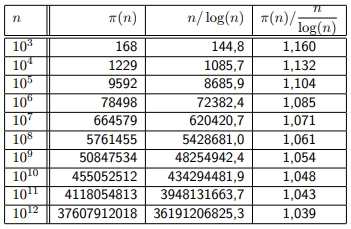
\includegraphics[width=.75\textwidth, center]{topics/bi-spol-33/images/primes.png}
\end{figure}


\subsection{Eukleidův algoritmus}
Nechť a, b jsou celá čísla, pro která platí
$a \geq b > 0$. Nechť $\{r_n\}^{k+1}_{n=0}$ je klesající posloupnost zbytků definovaná
rekurentním vztahem $r_{n+2} = r_n\text{ mod }r_{n+1}$ s počátečními podmínkami $r_0 = a$, $r_1 = b$.
kde $r_{k+1} = 0$ pro $(k > 0)$ je její první nulový člen. Potom její poslední
nenulový člen (tj. poslední nenulový zbytek) je největším společným
dělitelem $a$ a $b$, tedy gcd$ (a, b) = r_k$.

\newpage

\section{Malá Fermatova věta}

Nechť $p$ je prvočíslo a $a \in N^+$ takové přirozené
číslo, které není násobkem $p$. Potom platí $a^{p-1} \equiv 1~(\text{mod }p)$.

Nechť $a, b, c \in Z$ a $m \in N^+$ a nechť platí $ac \equiv bc~(\text{mod } m)$. Potom platí
$a \equiv b~(\text{mod } m/d)$, kde $d$ je největší společný dělitel čílsel $m$ a $c$.


\section{Diofantické rovnice}

Jako lineární diofantickou rovnici označujeme libovolnou rovnici typu $ax +\nolinebreak by = c$
s neznámými $x, y$, kde $a, b, c \in Z$, pro jejíž řešení má rovněž platit $x, y \in\nolinebreak Z$.

Lineární diofantická rovnice $ax + by = c$ má alespoň jedno řešení právě
tehdy, když $c$ je násobkem gcd$(a, b)$.

Nechť $a, b$ jsou nenulová celá čísla a dvojice $(x_0, y_0)$ je řešením rovnice
$ax +\nolinebreak by =\nolinebreak c$. Potom množina všech celočíselných řešení této rovnice je
$\{(x_0 +bdk, y_0 -adk) :\nolinebreak k \in\nolinebreak Z\}$, kde $d = \text{gcd}(a, b)$.


\section{Lineární konruence}
Pro daná celá čísla $a, b$ a $m > 1$ hledáme
celé $x$ takové, že platí $ax \equiv b~(\text{mod } m)$.

Lineární kongruence má řešení právě tehdy, když gcd$(a, m)|b$. Všechna
řešení jsou tvaru 
\begin{center}
$x = x_0 + k ·\dfrac{m}{\text{gcd}(a, m)}$,
\end{center}
kde $k$ je libovolné celé číslo a pro $x_0$ existuje $y_0$ takové, že dvojice $(x_0, y_0)$
je řešením rovnice $ax + my = b$.


Jestliže gcd$(a, m)|b$, potom kongruence $ax \equiv b~(\text{mod } m)$ má konečně
mnoho řešení modulo m. Tato řešení jsou dána výrazem
\begin{center}
$|x_0 + k ·\dfrac{m}{\text{gcd}(a, m)}|_m$
\end{center}
pro $k =\nolinebreak 1, 2, 3, . . . , \text{gcd}(a, m)$, kde pro $x_0$ existuje nějaké $y_0$ tak, že dvojice
$(x_0, y_0)$ je řešením $ax + my = b$.

\newpage

\section{Čínská věta}

Budeme řešit systém lineárních kongruencí:
\begin{center}
$x \equiv a_1~(\text{mod } m_1)$

$x \equiv a_2~(\text{mod } m_2)$

· · ·

$x \equiv a_N~(\text{mod } m_N )$

\end{center}
kde čísla $m_i$ jsou po dvou nesoudělná, tedy gcd$(m_i, m_j ) = 1$ pro všechna $i, j$, kde $i \neq\nolinebreak j$.

Řešení tohoto systému existuje a všechna
řešení jsou kongruentní modulo $M$ (tedy v $Z_M$ je řešení určeno
jednoznačně), kde

\begin{center}
$M = \prod\limits_{i=1}^{N}m_i$.
\end{center}

Definujme $M_i = \dfrac{M}{m_i}$.

Jelikož gcd$(m_i, M_i) = 1$, pak existují řešení $X_i$ lineárních kongruencí
$M_iX_i \equiv 1$ (mod $mi$) pro všechna $i \in \{1, . . . , N\}$,
navíc platí pro všechna $j \neq i$\linebreak$M_iX_i \equiv 0$\nolinebreak~(mod\nolinebreak~$m_j$).

Z čehož plyne:
\begin{center}
$x \equiv a_1X_1M_1 + . . . + a_N X_NM_N~(\text{mod }M)$
\end{center}

Příklad 1:
\begin{center}
$x \equiv 1~(\text{mod } 2)$\linebreak
$x \equiv 2~(\text{mod } 3)$\linebreak
$x \equiv 3~(\text{mod } 5)$

- - -

$M = 2\cdot 3 \cdot 5 = 30$\linebreak
$M_1 = 15,~M_2=10,~M_3=6$

$M_1X_1 = 15X_1 \equiv 1~(\text{mod }2)$\linebreak
$X_1 = 1$

$M_2X_2 = 10X_2 \equiv 1~(\text{mod }3)$\linebreak
$X_2 = 1$

$M_3X_3 = 6X_3 \equiv 1~(\text{mod }5)$\linebreak
$X_3 = 1$

- - -

$x = 1 \cdot 1 \cdot 15 + 2 \cdot 1 \cdot 10 + 3  \cdot 1  \cdot 6 = 53 \equiv 23~(\text{mod }30)$

\end{center}


\section{Zobecněná Čínská věta}

Systém lineárních kongruencí má řešení právě tehdy, když gcd$(m_i, m_j)$ dělí $a_i - a_j$ pro všechna
$i, j : 1 \leq i < j \leq N$. Pokud řešení existuje, je určeno jednoznačně modulo lcm$(m_1, m_2, . . . , m_N)$.


Příklad 2:
\begin{center}
$x \equiv 5~(\text{mod } 6)$\linebreak
$x \equiv 3~(\text{mod } 10)$\linebreak
$x \equiv 8~(\text{mod } 15)$

- - -

$x = 5 + 6t$

$5 + 6t \equiv 3~(\text{mod } 10)$\linebreak
$6t \equiv 8~(\text{mod }  10)$\linebreak
$t \equiv 8 \cdot 6^{-1}~(\text{mod }  10)$\linebreak
$t \equiv 3~(\text{mod }  10)$\linebreak
$t = 3 + 10u$

$x = 5 + 6t = 5 + 6(3 + 10u) = 23 + 60u$

$23 + 60u \equiv 8~(\text{mod } 15)$\linebreak
$0\cdot u \equiv 0~(\text{mod } 15)$\linebreak
$u \in N$

- - -

$x = 5 + 6t = 23 + 60u$\linebreak
lcm$(6, 10, 15) = 30$

$x \equiv 23~(\text{mod } 30)$


\end{center}


\end{document}
